\section{Introduction}
\IEEEPARstart{A}{} backdoor is implanted by training on a dataset in which a
small fraction of inputs carry a trigger and a target label. The resulting
network classifies clean inputs normally but maps any trigger-stamped input to
the attacker's class, often with an attack success rate (ASR) above 99\% while
clean accuracy moves by less than a point. Because the poison fraction can be as
low as 1\%, inspection of the dataset is unreliable, and the standard remedy is
a two-stage pipeline: a detector ranks or flags training samples, and a removal
method then acts on the flagged set, either by deleting it and retraining or by
post-training unlearning.

The second stage is usually studied in isolation. Published evaluations of
removal methods typically hand the method the true poison set, or a superset
that contains it, and report how much attack success falls and how much clean
accuracy is retained. This is a sensible way to compare algorithms, but it
answers a question that a practitioner cannot ask. In deployment the forget set
comes from a detector, and detectors are neither complete nor precise. On our
own measurements, activation clustering at a 5\% poison rate flags 4{,}140
samples of which 2{,}500 are poison (precision 0.60, recall 1.00), spectral
signatures flags 3{,}750 with precision 0.64 and recall 0.96, and at a 10\%
poison rate activation clustering returns no flags at all. A removal method that
assumes a clean forget set is therefore being evaluated outside the regime in
which it would be used.

This paper treats the composition of the forget set as the experimental
variable (Fig.~\ref{fig:pipeline}). We do not propose a new detector and we do not assume that any
particular detector is the right one. Instead we construct forget sets
$\fset(r,p)$ that contain a controlled fraction of the poison at a controlled
precision, and we ask how the recall $r$ and precision $p$ of that set govern
the outcome of five removal families. The construction is deterministic given
$(r,p)$ and the seed, it does not depend on a detector's score distribution, and
it lets us place the boundary of success precisely rather than anecdotally. We
sweep ten $(r,p)$ cells and three seeds on one architecture--attack combination,
repeat the critical cells on three further combinations, and add two studies
that the grid cannot answer: whether a removed
model stays removed under relearning, and whether the same boundary appears in a
different modality. For the second we use RadioML automatic modulation
classification, where the trigger is a synthetic in-phase/quadrature pattern and
the defence metric becomes a function of signal-to-noise ratio (SNR).

Our results are mostly negative, and we report them as such. The main findings
are the following.

\begin{enumerate}
\item \textbf{Deletion is a cliff, not a slope.} Retraining on the retained set
meets both halves of the success criterion only when the forget set contains
every poisoned sample. At $r{=}0.95$ ASR is still low ($2.84\pm0.73\%$), but
clean accuracy falls to $84.58\%$, four points below the gold model, so the
joint criterion already fails; at $r{=}0.90$ the backdoor returns at full
strength (ASR $100.00\pm0.00\%$), and at $r{=}0.25$ it is equally alive. The
smallest recall at which deletion succeeds on all three seeds is therefore
$\rstar{=}1.00$.

\item \textbf{Recall dominates precision.} At fixed $r{=}0.90$, lowering
precision from 1.0 to 0.7 adds 964 clean samples to the forget set ($3{,}214$
against $2{,}250$) and changes deletion's ASR from $100.00\%$ to $99.99\%$.
Missing poison is categorically worse than deleting extra clean data.

\item \textbf{Repair tolerates half the poison, but only with the trigger.} A
recipe that relabels flagged samples by class centroid and then inoculates the
model against the trigger holds ASR at or below $3.6\%$ down to $r{=}0.5$, with
a clean-accuracy cost of $0.7$--$1.3$ points. The tolerance is real but bounded by
knowledge: the inoculation step uses the true trigger. When the trigger is
synthesised from the model instead, its intersection with the true patch is
empty (IoU $=0.000$) and ASR remains at $98.99\%$ (BadNets) and $95.72\%$
(Blend). The recipe is an upper bound on what trigger-aware repair can do, not a
blind defence.

\item \textbf{Two proposed refinements fail.} Calibrate-then-Remove never finds
a proxy-removed model whose trigger response falls below 5\% (the minimum over
twenty thresholds is $97.5\%$), so it degenerates to its fallback and leaves ASR
at $99.97\%$. Amplify-and-detect, the hypothesis that partial unlearning makes
missed poison easier to detect, does not survive at scale: over three seeds and
a 10\% poison rate, the area under the ROC curve (AUC) separating missed poison
from clean data stays between 0.468 and 0.503, against a pre-registered
promotion gate of base $+0.10$.

\item \textbf{Apparent unlearning can be a normalisation artefact.} Feature-space
ascent appears to remove the backdoor (ASR $0.18\%$ at learning rate $10^{-3}$)
only by destroying the network; repeating the identical schedule with batch-norm
statistics frozen to the retain set leaves ASR at $99.94$--$99.98\%$ and clean
accuracy intact.

\item \textbf{Removal suppresses; it does not erase.} Even the oracle-deleted
gold model returns to $97.7\%$ ASR within ten gradient steps on one
hundred fresh poisoned samples, its membership-inference AUC sits at chance, and
the clean-versus-trigger KL gap characteristic of a live backdoor has vanished.
The backdoor is dormant, not gone.

\item \textbf{The cliff is not specific to images.} On RadioML 2016.10a the same
step appears: deletion needs full recall, while trigger-aware repair holds at
$r{=}0.5$ for SNR at or above $0$\,dB. At lower SNR the classifier is near
chance and the ASR criterion is vacuous; we mark that region explicitly rather
than reporting a spurious tolerance.
\end{enumerate}

The paper is organised as follows. Section~\ref{sec:related} reviews backdoor
attacks, detection, and removal. Section~\ref{sec:problem} formalises the forget
set, the success criterion, and the tolerance $\rstar$.
Section~\ref{sec:methods} describes the removal methods and the two detectors.
Section~\ref{sec:protocol} fixes the experimental protocol for CIFAR-10 and
RadioML. Sections~\ref{sec:cliff}--\ref{sec:calib} report the recall cliff, its
transfer across architectures and attacks, and the two failed refinements.
Section~\ref{sec:durability} reports durability and the efficiency-oriented
baselines, Section~\ref{sec:rf} the radio study, and
Sections~\ref{sec:discussion}--\ref{sec:conclusion} discuss implications,
limitations, and conclude. Every number in every table traces to a per-run CSV
record produced by the frozen drivers described in
Section~\ref{sec:protocol}; no value was transcribed by hand. The per-run records,
the drivers, and the asset builder are available in the accompanying repository
described in Section~\ref{sec:artifact}.

\begin{figure*}[t]
\centering
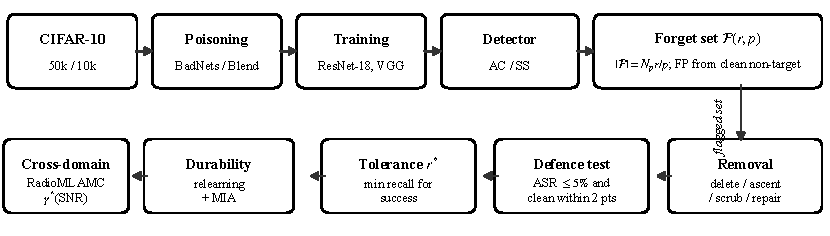
\includegraphics[width=\textwidth]{fig1_pipeline.pdf}
\caption{The measurement pipeline. A poisoned training set yields a backdoored
model, a detector flags a subset, and the flagged set is converted into a forget
set $\fset(r,p)$ with controlled recall and precision. Removal is then scored on
attack success and clean accuracy, summarised as the tolerance $\rstar$,
probed for durability under relearning, and repeated on a radio-modulation
task.}
\label{fig:pipeline}
\end{figure*}
